\documentclass{article}
\usepackage{tikz}
\usepackage{amsmath,amssymb}
\usetikzlibrary{arrows.meta, calc, backgrounds}

\begin{document}

\begin{figure}[htbp]
  \centering
  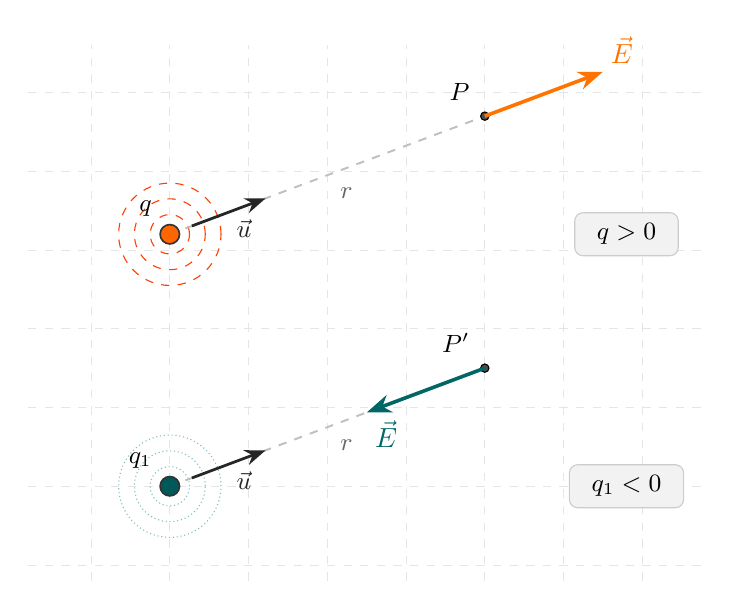
\begin{tikzpicture}[>=Stealth, font=\small\sffamily]

    % Stili grafici personalizzati
    \tikzset{
      gridline/.style={draw=gray!20, line width=0.3pt, dashed},
      badge/.style={draw=gray!40, fill=gray!10, rounded corners=3pt, inner xsep=8pt, inner ysep=4pt, font=\small\sffamily},
      fieldarrow/.style={line width=1.3pt, ->},
      posline/.style={draw=gray!50, line width=0.7pt, dashed},
      unitarrow/.style={line width=1.0pt, ->, color=black!85}
    }

    % Griglia tecnica di sfondo
    \draw[gridline] (-1.8,-2.2) grid (6.8,4.6);

    % ==========================================
    % CASO 1: Carica positiva (q > 0) - Campo uscente
    % ==========================================
    \coordinate (A1) at (0, 2.2);
    \coordinate (B1) at (4.0, 3.7);

    % Anelli concentrici di campo
    \foreach \r in {0.25, 0.45, 0.65} {
      \draw[orange!50!red, line width=0.4pt, dashed] (A1) circle (\r);
    }

    % Linea della distanza r
    \draw[posline] (A1) -- (B1) node[midway, below right=1pt, font=\small\itshape, color=gray!80!black] {$r$};

    % Versore u
    \draw[unitarrow] ($(A1)!0.3cm!(B1)$) -- ($(A1)!1.3cm!(B1)$) node[midway, below right=-1pt, font=\bfseries\small] {$\vec{u}$};

    % Punto P e vettore Campo Elettrico E (uscente)
    \filldraw[fill=black!70, draw=black] (B1) circle (1.5pt) node[above left=2pt, font=\small\itshape] {$P$};
    \draw[fieldarrow, color=orange!90!red] (B1) -- ($(B1)!-1.6cm!(A1)$) node[above right=-1pt, font=\bfseries] {$\vec{E}$};

    % Carica sorgente q
    \filldraw[fill=orange!80!red, draw=black!80, line width=0.6pt] (A1) circle (3.5pt);
    \node[above left=3pt, font=\small\bfseries] at (A1) {$q$};

    % Badge identificativo della condizione
    \node[badge] at (5.8, 2.2) {$q > 0$};


    % ==========================================
    % CASO 2: Carica negativa (q1 < 0) - Campo entrante
    % ==========================================
    \coordinate (A2) at (0, -1.0);
    \coordinate (B2) at (4.0, 0.5);

    % Anelli concentrici di campo
    \foreach \r in {0.25, 0.45, 0.65} {
      \draw[teal!50, line width=0.4pt, densely dotted] (A2) circle (\r);
    }

    % Linea della distanza r
    \draw[posline] (A2) -- (B2) node[midway, below right=1pt, font=\small\itshape, color=gray!80!black] {$r$};

    % Versore u
    \draw[unitarrow] ($(A2)!0.3cm!(B2)$) -- ($(A2)!1.3cm!(B2)$) node[midway, below right=-1pt, font=\bfseries\small] {$\vec{u}$};

    % Punto P' e vettore Campo Elettrico E (entrante)
    \filldraw[fill=black!70, draw=black] (B2) circle (1.5pt) node[above left=2pt, font=\small\itshape] {$P'$};
    \draw[fieldarrow, color=teal!80!black] (B2) -- ($(B2)!1.6cm!(A2)$) node[below right=-1pt, font=\bfseries] {$\vec{E}$};

    % Carica sorgente q1
    \filldraw[fill=teal!70!black, draw=black!80, line width=0.6pt] (A2) circle (3.5pt);
    \node[above left=3pt, font=\small\bfseries] at (A2) {$q_1$};

    % Badge identificativo della condizione
    \node[badge] at (5.8, -1.0) {$q_1 < 0$};

  \end{tikzpicture}
  \caption{Orientazione del campo elettrostatico $\vec{E}$ nel punto di misura per una carica sorgente positiva $q$ ed una carica negativa $q_1$.}
  \label{fig:campo_carica_puntiforme_infografica}
\end{figure}

\end{document}